\documentclass{beamer}
\usetheme{Copenhagen}
% \usepackage{metropolis_framesubtitle}
\usepackage[]{mathtools}
\definecolor{UBCblue}{rgb}{0.04706, 0.13725, 0.26667} % UBC Blue (primary)
\usecolortheme[named=UBCblue]{structure}
% \setbeamercolor{frametitle}{bg=black}
% \usefonttheme[]{serif}
% \usecolortheme{spruce}

\title[Lattices and Number Theory]{Can lattice points approximate irrationals?}
\subtitle[]{Exploring number theory through the regular system of points}
\author[Abhisruta Maity]{Abhisruta Maity}
\institute{21MS, IISER Kolkata}
\date{July 4, 2022}
\setbeamertemplate{title page}[default][colsep=-4bp,rounded=true]

\begin{document}
    \begin{frame}
        \titlepage
    \end{frame}

    \begin{frame}
        \frametitle{A look into lattice points}
        \framesubtitle{a.k.a. regular system of points in a plane}
        \begin{figure}
            \includegraphics[scale=0.40]{latt.png}
        \end{figure}

    \end{frame}
    \begin{frame}
        \frametitle{Generating lattice structure}
        \framesubtitle{Hero: Unit cells}
        \begin{columns}
            \column{0.5\textwidth}
                A square can generate a square lattice. A parallelogram can generate a square lattice too. These fundamental geometric objects which generate the lattice are called unit cells. \\~\\

                A lattice can be generated by square or parallelogram shaped unit cells having some specific shapes. Thus, given any lattice structure, the unit cell corresponding to it is not unique.
            \column{0.5\textwidth}
                \begin{figure}
                    \centering
                    \includegraphics[scale=0.20]{unit.png}
                \end{figure}
        \end{columns}
    \end{frame}

    \begin{frame}
        \frametitle{Circle entered the room \\ \footnotesize Hunting lattice points inside a circle}
        \framesubtitle{}
        \begin{figure}
            \includegraphics[scale=0.20]{scene1.png}
        \end{figure}
    \end{frame}

    \begin{frame}
        \frametitle{Circle entered the room}
        \framesubtitle{Approximating the area of the circle through lattice points}
        \begin{figure}
            \includegraphics[scale=0.20]{scene2.png}
        \end{figure}
    \end{frame}

    \begin{frame}
        \frametitle{Approximating the area}
        \framesubtitle{\(\pi\): I am coming!}
        \begin{figure}
            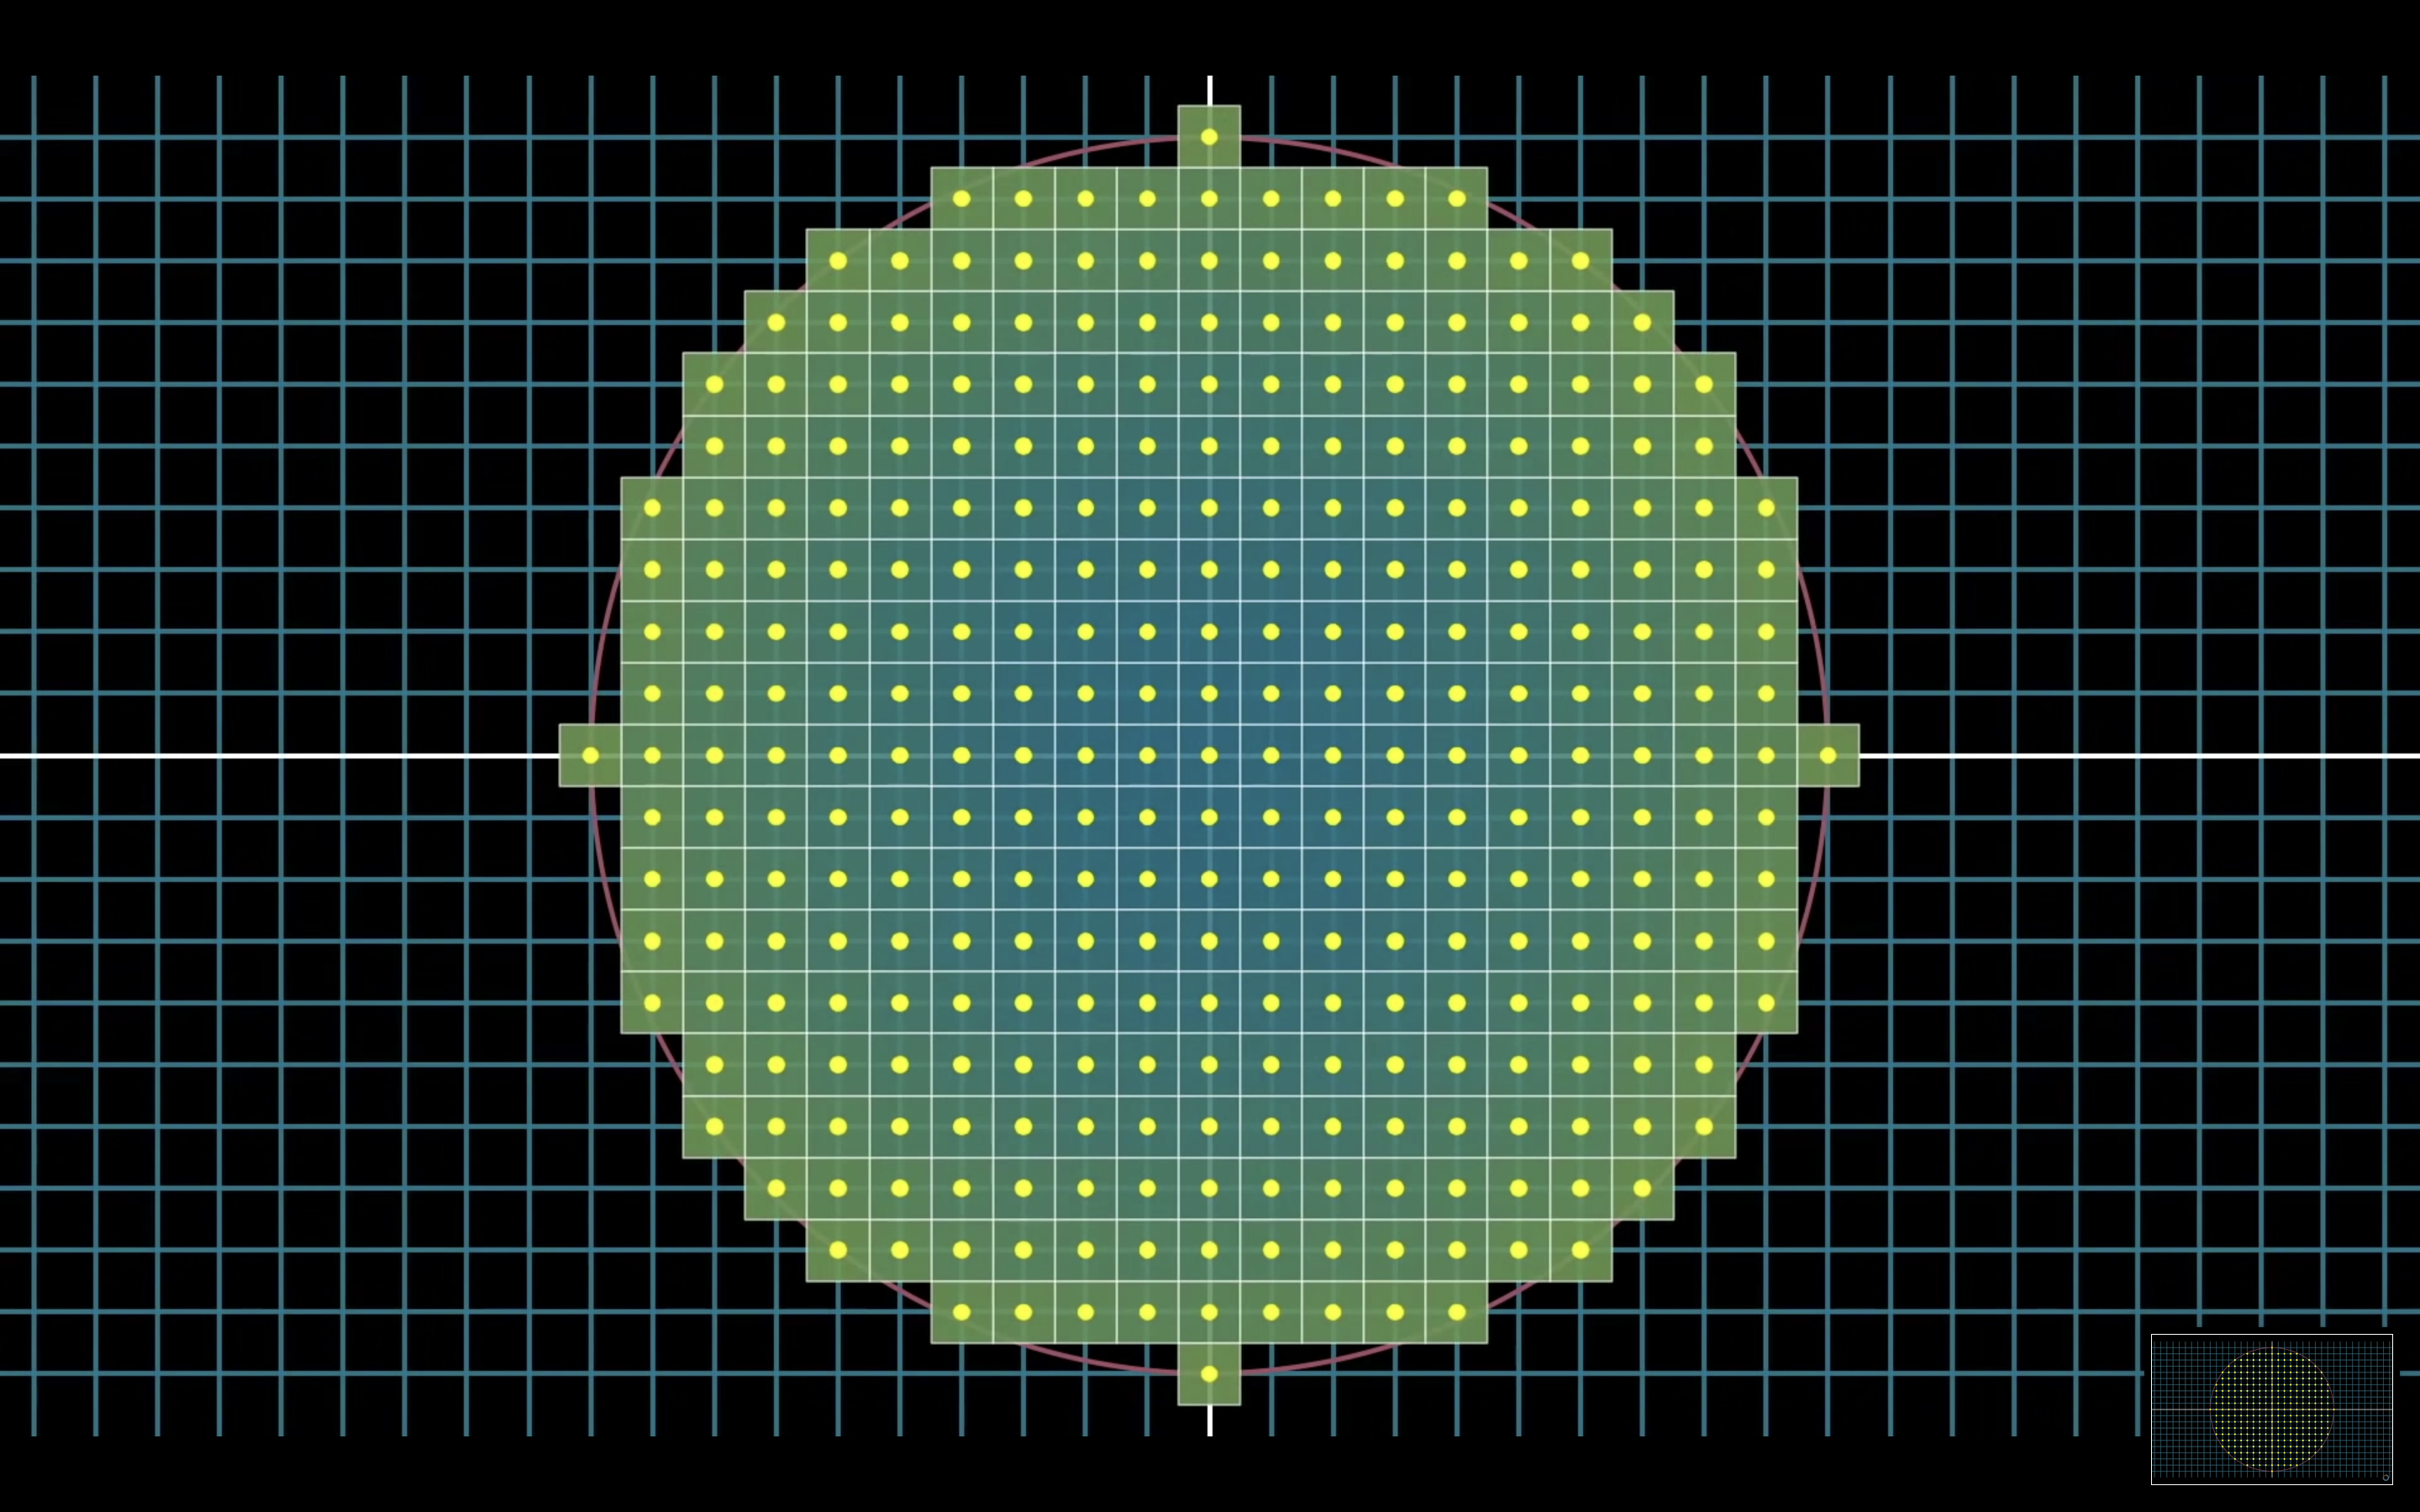
\includegraphics[scale=0.20]{scene3.png}
        \end{figure}
    \end{frame}

    \begin{frame}
        \frametitle{Is it a good approximation?}
        Suppose we assign the lattice points integer coordinates. Let the number of lattice points inside and on the circle is \(N(r)\) for a given integer radius \(r\). We estimate \[|\pi r^2 - N(r)| < \varepsilon(r)\] If \(\varepsilon(r)\) is negatively correlated with \(r\) then we are sure that this is indeed a good approximation. \\~\\

        This is the time we have to look back the previous diagram to estimate or find some bound on \(\varepsilon(r)\).
    \end{frame}

    \begin{frame}
        \frametitle{The bad squares}
        \framesubtitle{Can we estimate the area of the bad squares which is yielding the error?}
        \begin{figure}
            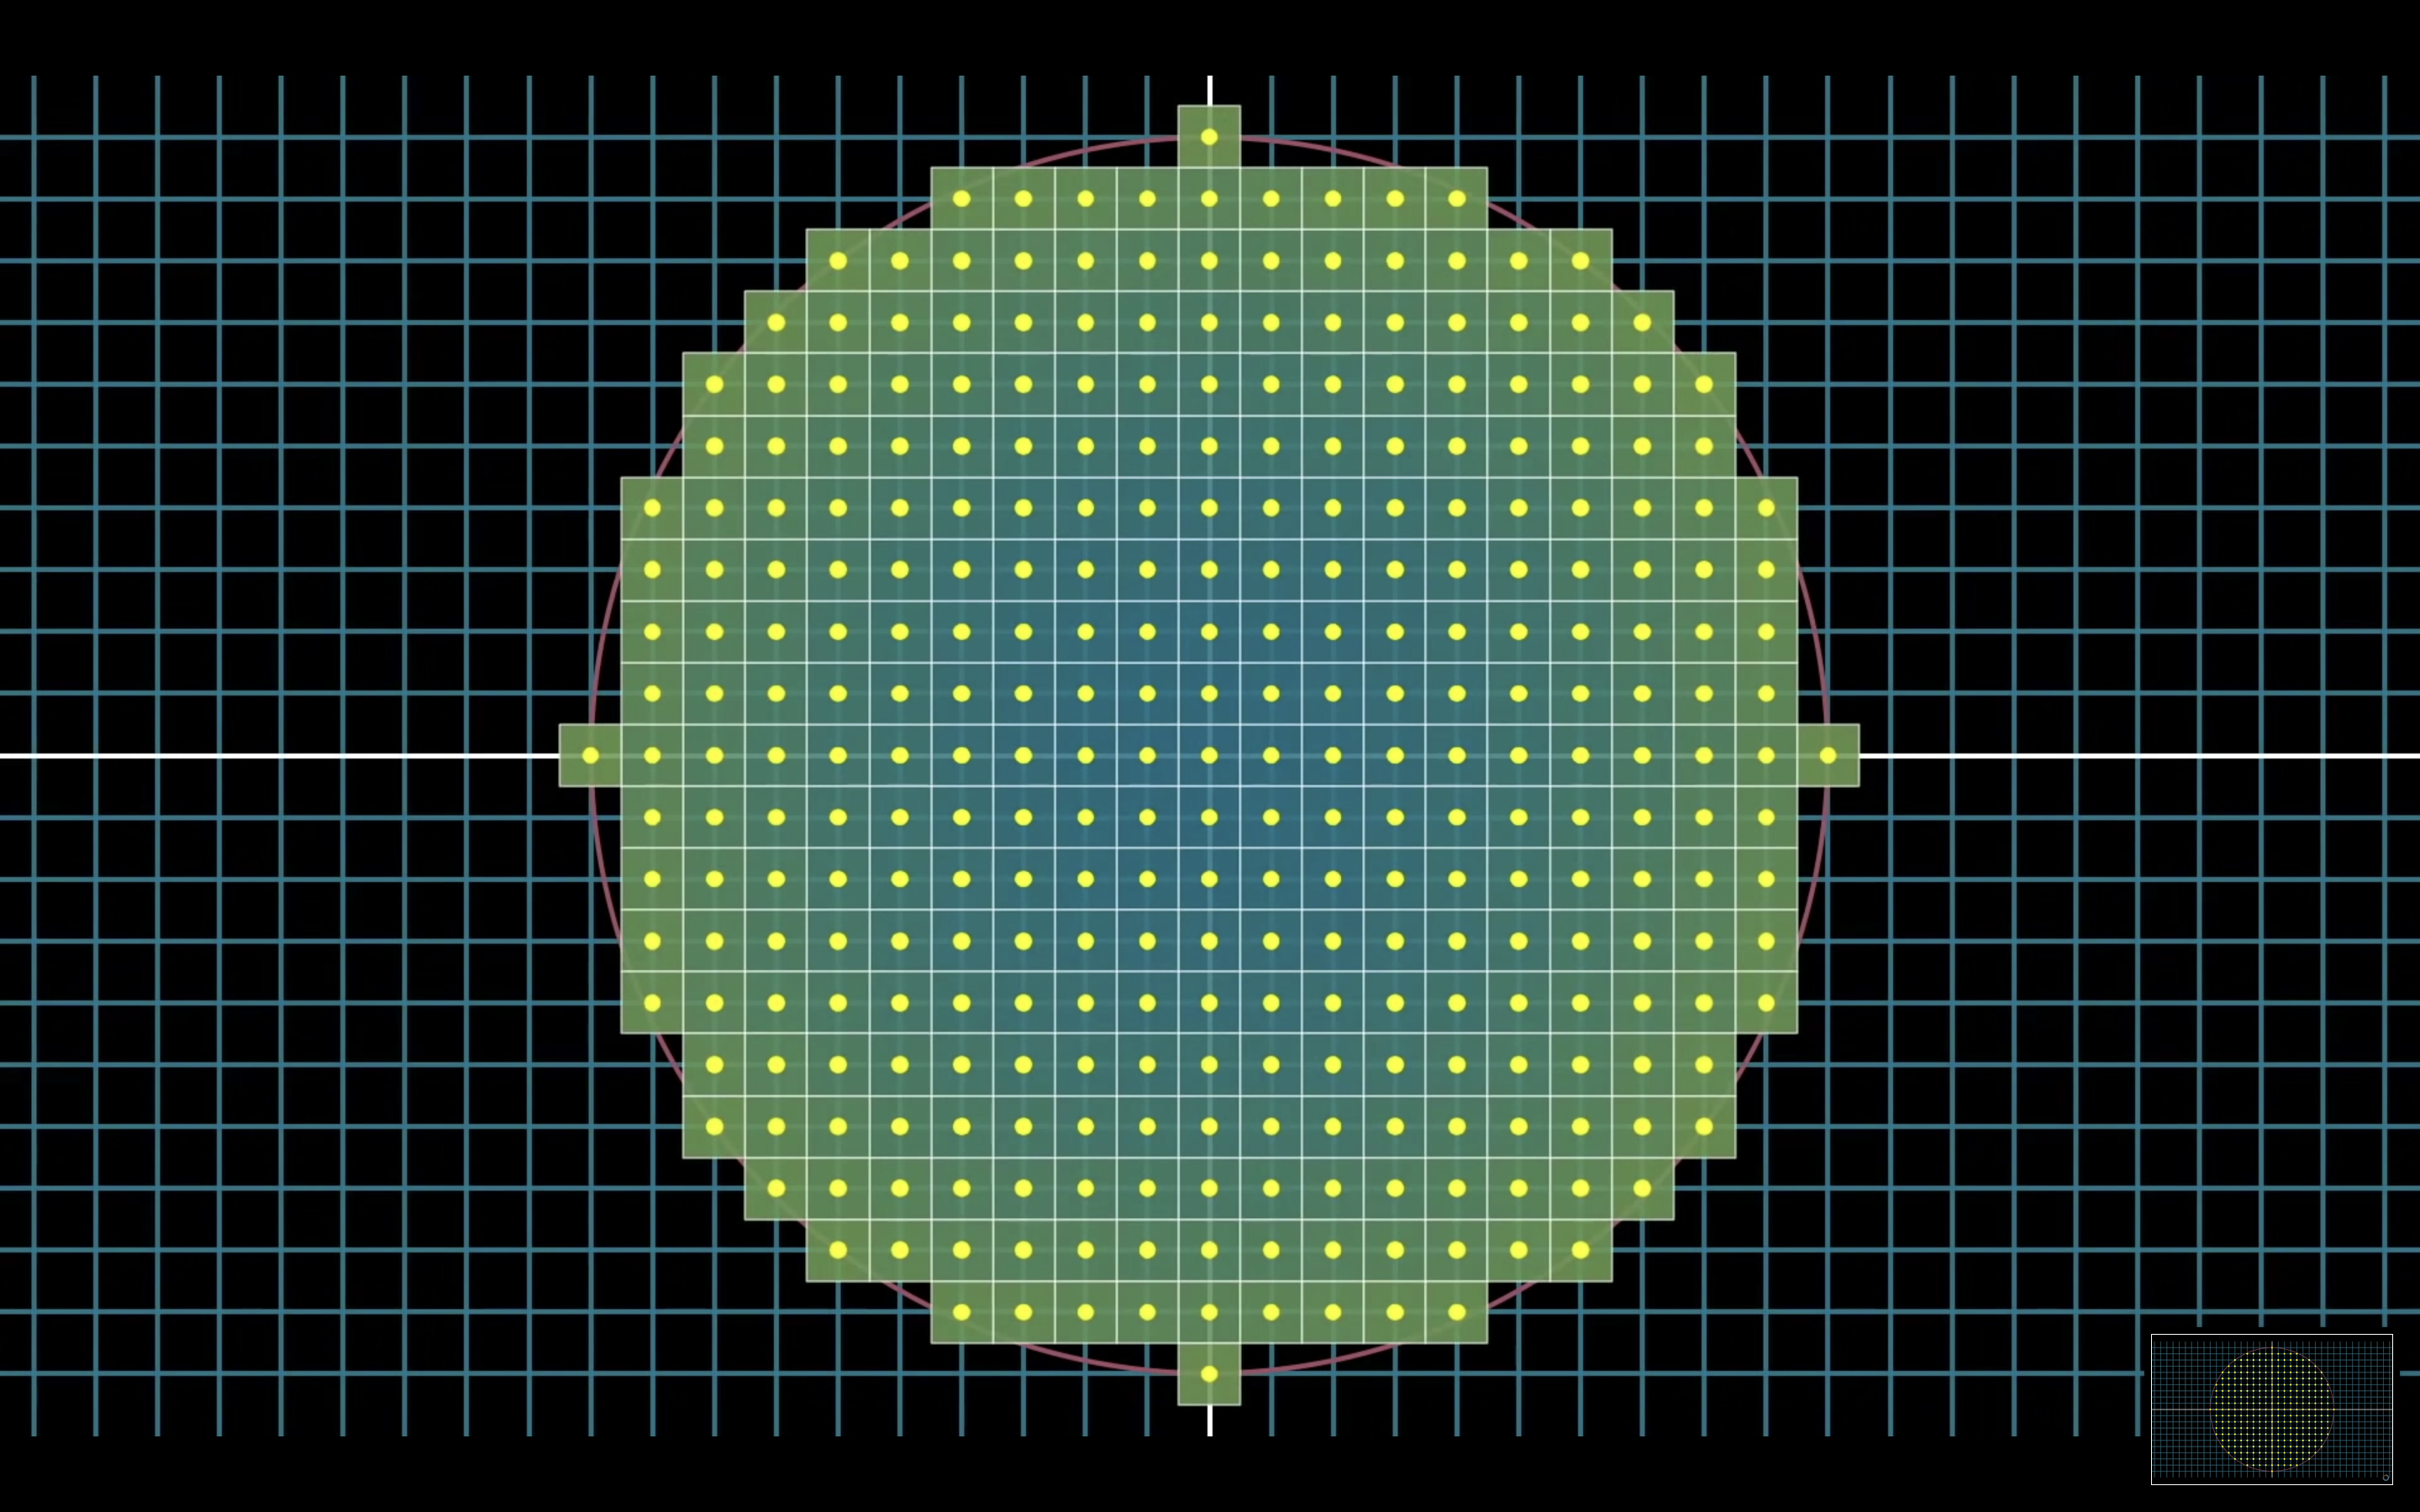
\includegraphics[scale=0.20]{scene3.png}
        \end{figure}
    \end{frame}

    \begin{frame}
        \frametitle{Estimating the bad area}
        The bad squares are entirely contained inside the annulus of smaller radius \(r - \sqrt{2}\) and bigger radius \(r + \sqrt{2}\). Hence the bad area \[\varepsilon(r) < E(r) = \pi [(r+\sqrt{2})^2 - (r-\sqrt{2})^2] = 4 \sqrt{2} \pi r\] Now it's moment to plug back!
    \end{frame}

    \begin{frame}
        \frametitle{Contd.: Is it a good approximation?}
        Our previous estimation then becomes \[|\pi r^2 - N(r)| < \varepsilon(r) < 4 \sqrt{2} \pi r\] Dividing by \(r^2\) yields \[\left|\pi - \frac{N(r)}{r^2}\right| < \frac{4 \sqrt{2} \pi}{r}\] Look at the equation: \(N(r), r \in \mathbb{N}\). Hence, \(\frac{N(r)}{r^2}\) is a rational approximation of the irrational number \(\pi\) with the fact that we can approximate as close as we want, with increasing \(r\), subsequently decreasing the error term.
    \end{frame}

    \begin{frame}
        \frametitle{\(\sqrt{2}, e\) : What about approximating us?}

        Before diving into it, let's do some other works: deduce some important properties of the lattice structure. \\~\\

        Specifically, we will take ``unit lattices'' into account. Unit lattices are the lattice structures which are generated by the parallelograms or squares whose area is 1 unit\(^2\). 
    \end{frame}

    \begin{frame}
        \frametitle{Story of unit lattices}
        Did you all remember the `solid state' chapter in +2 grade? We will talk about a concept we have learned in there, i.e., ``The distance of a lattice point to its first neighbour (denote that distance as \(c\))''. \\~\\

        Suppose, you have a unit lattice structure. What is the minimum value of \(c\)? Clearly, if we shear the unit cell parallelogram such that area remains 1 unit\(^2\), then \(c\) can be made arbitrarily small as a side of the parallelogram, forcing another side to be arbitrarily large \(\frac{1}{c}\). So, making \(c\) small is not that interesting. But is there any constraint in making \(c\) large, in other words, what is the maximum possible value of \(c\) for a unit lattice?
    \end{frame}

    \begin{frame}
        \frametitle{Finding max of the min distance}
        \begin{figure}
            \includegraphics[scale=0.45]{dist.png}
        \end{figure}
    \end{frame}

    \begin{frame}
        \frametitle{Contd.: Finding max of the min distance}
        In any given unit lattice, choose any pair of lattice points the distance between which is the minimum distance \(c\). On the straight lineg passing through these two points there must, according to the definition of the lattice, be infinitely many more lattice points spaced at intervals of length \(c\). The straight line \(h\) that is parallel tog and at a distance \(\frac{1}{c}\) from it must also contain infinitely many lattice points, but the strip betweeng and h cannot contain any. We now draw circles of radius \(c\) about all the lattice points on \(g\). The totality of circles covers a strip of the plane bounded by circular arcs. Every interior point of this strip is less than \(c\) distant from at least one lattice point and therefore, by the definition of \(c\), is not itself a lattice point. Hence \(\frac{1}{c}\) is greater than or equal to the shortest distance between the boundary of the strip and \(g\). Evidently this distance is the altitude of an equilateral triangle of side \(c\).
    \end{frame}

    \begin{frame}
        \frametitle{Contd.: Finding max of the min distance}
        Thus we have, \[\frac{1}{c} \geq \frac{c}{2}\sqrt{3}\] which yields an upper bound: \[c \leq \sqrt{\frac{2}{\sqrt{3}}}\]
        An easy exercise is to check when does the equality occur!
    \end{frame}

    \begin{frame}
        \frametitle{Approximation back again!}
        \framesubtitle{Focusing object: Quadratic forms}
        Consider the quadratic form of two variables \[Q(x,y) = ax^2 + 2hxy + by^2\] where \(a,h,b \in \mathbb{R}\). Inspecting \(Q(x,y)\), we get a representation of it in the following way: \[Q(x,y) = \begin{bmatrix}
            x & y
        \end{bmatrix}
        \begin{bmatrix}
            a & h \\
            h & b
        \end{bmatrix}
        \begin{bmatrix}
            x \\
            y
        \end{bmatrix}\]
        The matrix in between is called \emph{Determinant} (denoted by \(D\)) of \(Q(x,y)\). For our problem, set \(D = 1\). Then \(a \neq 0\). WLOG, assume \(a > 0\).
    \end{frame}

    \begin{frame}
        \frametitle{Setting up an affine transformation}
        Notice that, now \(Q(x,y)\) can be written as \[Q(x,y) = \left(\sqrt{a}x + \frac{h}{\sqrt{a}}y\right)^2 + \left(\frac{1}{\sqrt{a}}y\right)^2\]
        Now set 
        \begin{align*}
            X &= \sqrt{a}x + \frac{h}{\sqrt{a}}y \\
            Y &= \frac{1}{\sqrt{a}}y
        \end{align*}
        Note that, this is an affine transformation with determinant 1 (thus, area scaled is 1, i.e., the unit cell square is sheared into a parallelogram), pictorially shown in the next slide.
    \end{frame}

    \begin{frame}
        \frametitle{The shear}
        \begin{figure}
            \includegraphics[scale=0.29]{shear.png}
        \end{figure}
        Ignore the parameters in the diagrams.
    \end{frame}

    \begin{frame}
        \frametitle{Contd.: The shear}
        If we allow \(x,y\) to run over integers (i.e., the pre-image lattice is ordinary unit square lattice), then the equation of the transformations represent set of points lying on the line \[X = h Y + \sqrt{a}m\] and \[Y = \frac{1}{a}n\] where \(m, n \in \mathbb{Z}\). Which roughly looks like the dots in the above diagram. Now, \[Q(x,y) = X^2 + Y^2\] Thus \(\sqrt{Q(x,y)}\) represents the distance from the origin to the point \((X,Y)\). The above ``first neighbour distance'' bound says that there will exist a point with the minimum distance \(c \leq \sqrt{\frac{2}{\sqrt{3}}}\).
    \end{frame}

    \begin{frame}

        \frametitle{Key lemma}

        Now, \[Q(x,y) = X^2 + Y^2\] Thus \(\sqrt{Q(x,y)}\) represents the distance from the origin to the point \((X,Y)\). The above ``first neighbour distance'' bound says that there will exist a point with the minimum distance \(c \leq \sqrt{\frac{2}{\sqrt{3}}}\). \\~\\
        
        Which in other words, there will always exist \(x,y \in \mathbb{Z}\) such that \[Q(x,y) \leq \frac{2}{\sqrt{3}}\].
    \end{frame}

    \begin{frame}
        \frametitle{The final bash}

        Let \(\epsilon > 0\). Consider the quadratic form \[Q(x,y) = \left(\frac{\alpha y - x}{\epsilon}\right)^2 + \epsilon^2y^2\] whose determinant is \[\frac{1}{\epsilon^2}\left(\frac{\alpha^2}{\epsilon^2} + \epsilon^2\right) - \frac{\alpha^2}{\epsilon^4} = 1\] From the above proved theorem it follows that, \(\exists x,y \in \mathbb{Z}\) such that \[Q(x,y) = \left(\frac{\alpha y - x}{\epsilon}\right)^2 + \epsilon^2y^2 \leq \frac{2}{\sqrt{3}}\] Consequently, as a \emph{fortiori} we have two simultaneous inequalities (projection of radius is lesser than or equal to the radius!): \[\left|\frac{\alpha y - x}{\epsilon}\right| \leq \sqrt{\frac{2}{\sqrt{3}}}, \quad |\epsilon y| \leq \sqrt{\frac{2}{\sqrt{3}}}\]
    \end{frame}

    \begin{frame}
        \frametitle{Contd.: The final bash}
        Rearranging the inequalities a bit, we have \[\left|\alpha - \frac{x}{y}\right| \leq \frac{\epsilon}{|y|}\sqrt{\frac{2}{\sqrt{3}}}, \quad |y| \leq \frac{1}{\epsilon}\sqrt{\frac{2}{\sqrt{3}}}\] Suppose \(\alpha\) is irrational. Then LHS of the left inequalities must be positive. Since \(\epsilon\) was arbitrary, we can obtain infinitely many pairs of \((x,y)\) setting \(\epsilon\) smaller and smaller, which forces the error in approximating \(\alpha\) by \(\frac{x}{y}\) \[\left|\alpha - \frac{x}{y}\right| \to 0\] Thus through this in the decreasing \(\epsilon\) process, we generate a sequence of \((x,y)\) which approximates irrational \(\alpha\), as precise as we desire. 
    \end{frame}

    \begin{frame}
        \frametitle{Contd.: The final bash}
        On other side of the process, we have the concise inequality \[\left|\alpha - \frac{x}{y}\right| \leq \frac{2}{\sqrt{3}} \frac{1}{y^2}\] which informs that rather a good approximation can be obtained by the sequence of \((x,y)\) with comparatively small denomenators, since the error is inversely proportional to square of the denomenator. \\~\\

        This turns out to be a little bit weaker version of the \emph{Dirichlet's Approximation theorem}, where the error bound has only the inverse of square of the denomenator.
    \end{frame}
\end{document}